\chapter{Message-oriented communication}
\subsubsection{Cosa vedremo in questa sezione}
Message-oriented communication:
\begin{itemize}
    \item The Web and HTTP messages
    \item Messages communication vs stream communication
\end{itemize}
Communication types
\begin{itemize}
    \item Synchronous and asynchronous communication
    \item Persistent and volatile communication
    \item Queue-based communication
\end{itemize}

\section{L'architettura del Web}
Il Web supporta l'interazione tra client e server via HTTP.
\begin{center}
    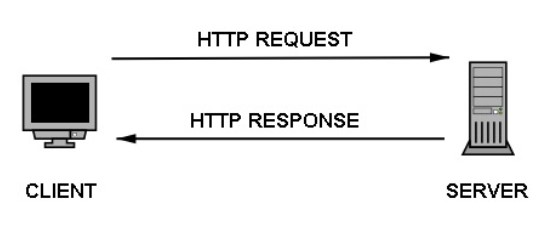
\includegraphics[width=0.675\textwidth]{img/MOC_architetture1.jpg}
\end{center}
Il client è realizzato da un “Browser” o “User-Agent”
\\Il server è realizzato da un “Web Server” o “HTTP Server”

\subsection{Il browser}
Il browser è l'applicazione per il Web sul lato del client.
\\Un web browser (detto User-Agent) è un programma che consente la navigazione nel Web da parte di un utente.
\\La funzione primaria di un browser è quella di interpretare il codice con cui sono espresse le informazioni (pagine web) e visualizzarlo (operazione di rendering) in forma di ipertesto.
\begin{itemize}
    \item I browser moderni hanno anche funzioni più avanzate per
    \\- trattare altri tipi di dati: es. Multimedialità, RSS, XML, JSON …
    \\- ospitare ed eseguire applicazioni: es. JavaScript (vedremo più avanti)
    \item Il rendering dipende dal dispositivi utilizzati, anche “non visuali”, ad esempio per supportare utenti non vedenti, es.:
    \\- sintesi vocale
    \\- alfabeto Braille
    \\...
\end{itemize}

\subsection{Web Page}
Una pagina web (web page, o anche documento) è costituita da diversi oggetti (risorse nella terminologia del web).
\\Una risorsa è un file, cioè una sequenza di dati (in formato digitale) residente in un computer, che è identificato da una URL (cioè un indirizzo univoco per la risorsa).
\begin{itemize}
    \item Testo, immagini, musica, …
\end{itemize}
La maggior parte delle pagine web sono costituite da un file HTML che definisce la struttura e i contenuti della pagina, testuali più altri oggetti.
\begin{itemize}
    \item HTML: HyperText Markup Language, è il linguaggio con cui si scrivono gli ipertesti (si definisce la struttura di una pagina, i collegamenti, si inseriscono immagini, …)
\end{itemize}
Un Web Server è una applicazione che si occupa di gestire le risorse (file) su un computer e di renderle disponibili ai client.

\subsection{Gli ipertesti}
Un ipertesto (hypertext) è un insieme di testi o pagine leggibili con l'ausilio di un'interfaccia elettronica, in maniera non sequenziale, tramite hyperlink (o più semplicemente link, cioè collegamenti), che costituiscono un rete raggiata o variamente incrociata di informazioni organizzate secondo criteri paritetici o gerarchici (es. menu).
\begin{center}
    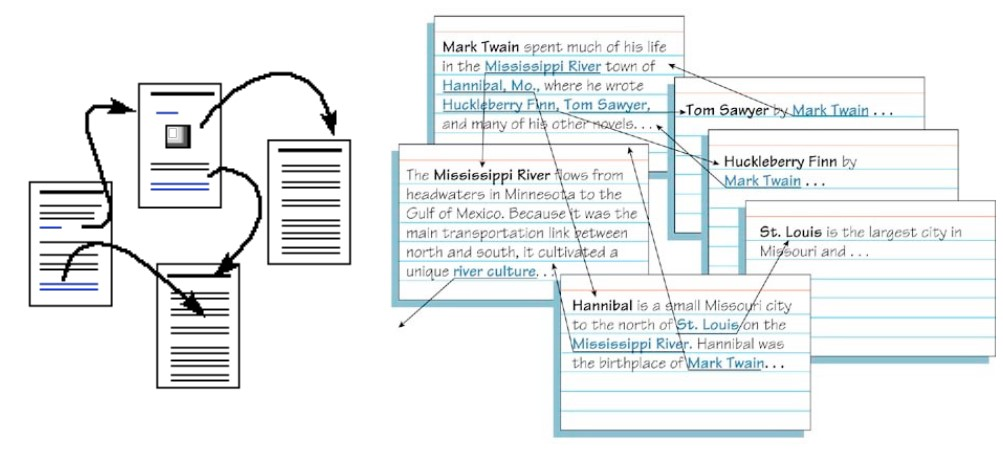
\includegraphics[width=0.675\textwidth]{img/MOC_architetture2.jpg}
\end{center}

\subsection{URL(Uniform Resource Locator)}
Identifica un oggetto nella rete e specifica come interpretare i dati ricevuti attraverso il protocollo.
\\Ha cinque componenti principali:
\begin{enumerate}
    \item nome del protocollo
    \item indirizzo dell'host
    \item porta del processo (la controparte)
    \item percorso nell'host
    \item Identificatore della risorsa
\end{enumerate}
\begin{verbatim}
    protocollo://indirizzo_IP[:porta]/cammino/risorsa
          1.          2.         3.      4.      5.
    ftp://www.adobe.com/dawnload/acroread.exe
    http://www.biblio.unimib.it/go/Home/Home-English/Services
    http://www.biblio.unimib.it/link/page.jsp?id=47502837
    http://www.someSchool.edu/someDept/pic.gif
    http://www.someSchool.edu:80/someDept/pic.gif
\end{verbatim}

\subsection{I linguaggi del Web}
I dati testuali sono espressi in linguaggi standard:
\begin{itemize}
    \item HTML (per definire la struttura dei contenuti e la loro impaginazione)
    \item può contenere CSS (per gestire la presentazione, cioè il rendering), …
    \item XML (focalizzato sui dati e la loro struttura)
    \item XSL, RDF, …
    \item JSON (focalizzato sui dati e la loro struttura)
\end{itemize}
I dati possono essere non testuali (immagini, audio, video)
\begin{itemize}
    \item Encoding MIME (definisce il formato dei contenuti)
\end{itemize}
La pagine Web possono contenere del codice espresso in linguaggi di scripting per arricchire l'interazione e rendere le pagine attive
\begin{itemize}
    \item JavaScript, VBScript, Java/Applet, Adobe Flash …
\end{itemize}

\section{Protocollo HTTP}
\subsection{Il concetto di protocollo}
Per poter capire le richieste e formulare le risposte i due processi devono concordare un protocollo.
% $\begin{definition}[Protocollo]
\\I protocolli definiscono il formato, l'ordine di invio e di ricezione dei messaggi tra i dispositivi, il tipo dei dati e le azioni da eseguire quando si riceve un messaggio.
% \end{definition}$
Esempi di protocollo
\begin{itemize}
    \item HTTP - HyperText Transfer Protocol
    \item FTP - File Transfer Protocol
    \item SMTP - Simple Mail Transfer Protocol
\end{itemize}
\begin{center}
    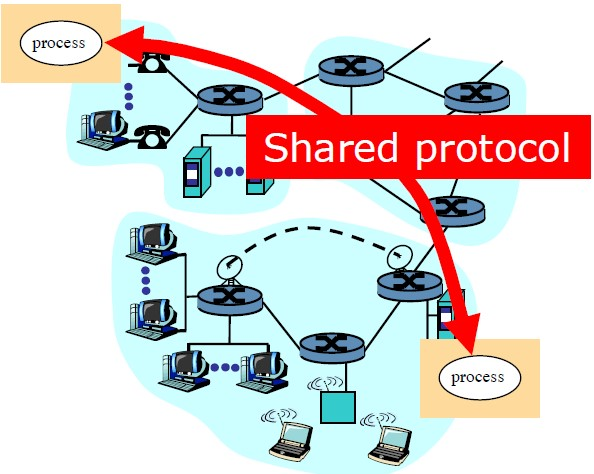
\includegraphics[width=0.675\textwidth]{img/MOC_protocolli1.jpg}
\end{center}

\subsection{Il Web: protocollo http}
http: hypertext transfer protocol
\\Protocollo di livello applicativo per il Web
\\Usa il modello client/server
\begin{itemize}
    \item client: browser che richiede, riceve e “mostra” oggetti Web
    \item server: Web server che invia oggetti in risposta alle richieste
\end{itemize}
\begin{center}
    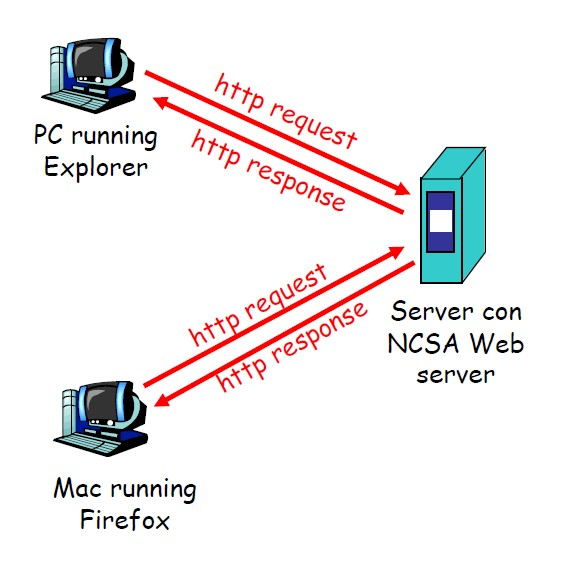
\includegraphics[width=0.5\textwidth]{img/MOC_protocolli2.jpg}
\end{center}
http1.0: RFC 1945
\\http1.1: RFC 2068

\subsubsection{http usa TCP}
Il client inizia una connessione TCP (crea una socket) verso il server sulla porta 80.
\\Il server accetta la connesione TCP dal client
\\Vengono scambiati messaggi http (messaggi del protocollo di livello applicativo) tra il browser (client http) e il Web server (server http).

\subsubsection{http è "stateless"}
Il server non mantiene informazione sulle richieste precedenti del client.
\\Quindi: ogni richiesta deve contenere tutte le informazioni necessarie per la sua esecuzione.
\\I protocolli che mantengono informazione di stato sono complessi (es. TCP)!

\subsection{Formato dei messagi http}
Due tipi di messaggi http: \textbf{\textit{request}}, \textbf{\textit{response}}.
\begin{itemize}
    \item ASCII (formato testo leggibile)
    \item Hanno la stessa struttura!
\end{itemize}
\begin{center}
    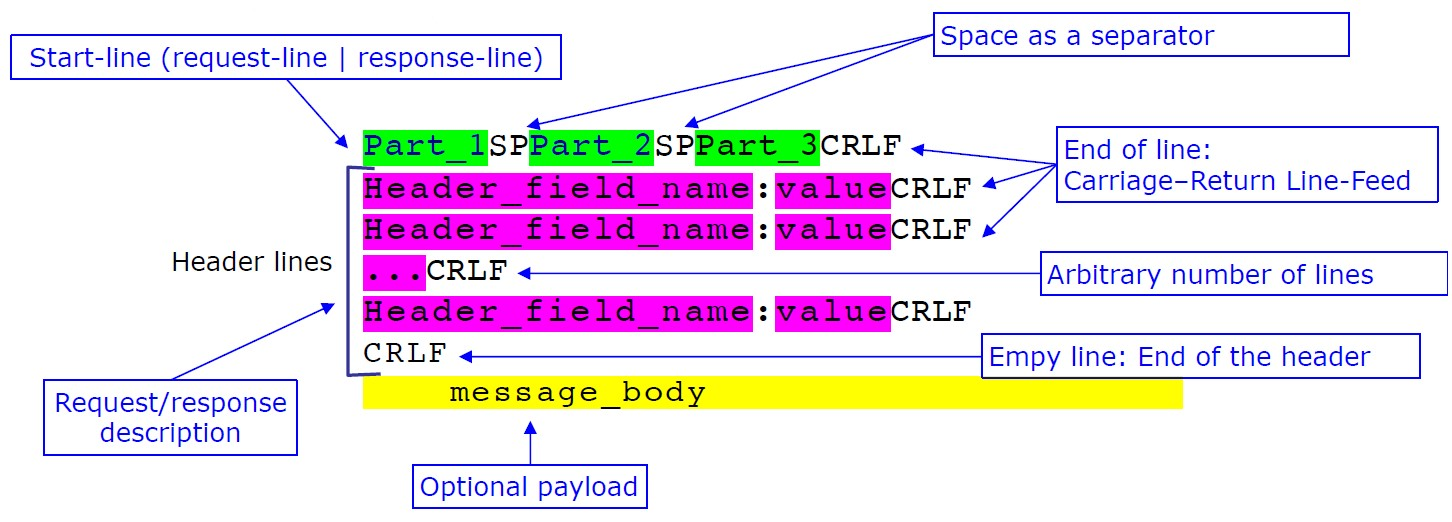
\includegraphics[width=0.5\textwidth]{img/MOC_messaggi1.jpg}
\end{center}
Messaggio http request
\begin{center}
    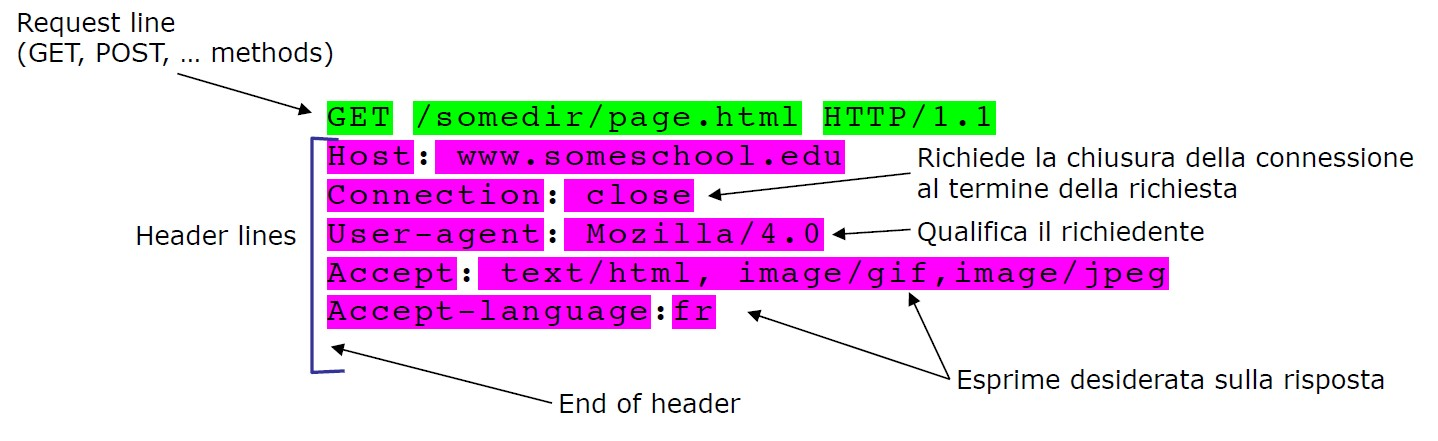
\includegraphics[width=0.5\textwidth]{img/MOC_messaggi2.jpg}
\end{center}

\subsection{Metodi e applicazioni web}
I principali metodi utilizzati sono:
\subsubsection{Metodo GET}
\begin{itemize}
    \item Restituisce una rappresentazione di una risorsa
    \item Include eventuali parametri in coda alla URL della risorsa (vedi più avanti)
    \item \`E safe: l'esecuzione non ha effetti sul server => la risposta può essere gestita con una cache dal client
    \item Uso tipico: ottenere dati in formato di pagine html e immagini, dati XML o JSON
\end{itemize}
La GET include eventuali parametri in coda alla URL della risorsa
\begin{verbatim}
    GET resource[?key=value{&key=value}] HTTP1.1
    {header lines}
\end{verbatim}
Esempio: dammi tutti gli ordini di marzo per il prodotto con codice Q2345
\begin{verbatim}
    /myCompany/orders?item="Q2345"&date="2022/03"
\end{verbatim}
\subsubsection{Metodo POST}
\begin{itemize}
    \item Comunica dei dati da elaborare lato server o crea una nuova risorsa subordinata all'URL indicata (vedi più avanti)
    \item L'input segue come documento autonomo (body)
    \item Non è idempotente: ogni esecuzione ha un diverso effetto => La risposta NON può essere gestita con una cache dal client
    \item Uso tipico: processare FORM e modificare dati in un DB
\end{itemize}
La POST prevede l'input in coda come documento autonomo (body)
\begin{verbatim}
    POST resource HTTP1.1
    {header lines}
    Body
\end{verbatim}
Esempio: aggiorna i codici di un prodotto in tutti gli ordini di aprile
\begin{verbatim}
    POST /myCompany/orders HTTP1.1
    {header lines}
    update=true&oldItem="Q2345"&newItem="Q68254"&date="2022/04"
\end{verbatim}
\subsubsection{Metodo HEAD}
\begin{itemize}
    \item Simile al metodo GET ma viene restituito solo l'Head della pagina Web
    \item Spesso usato in fase di debugging
\end{itemize}

\subsection{Metodi HTTP}
\begin{center}
    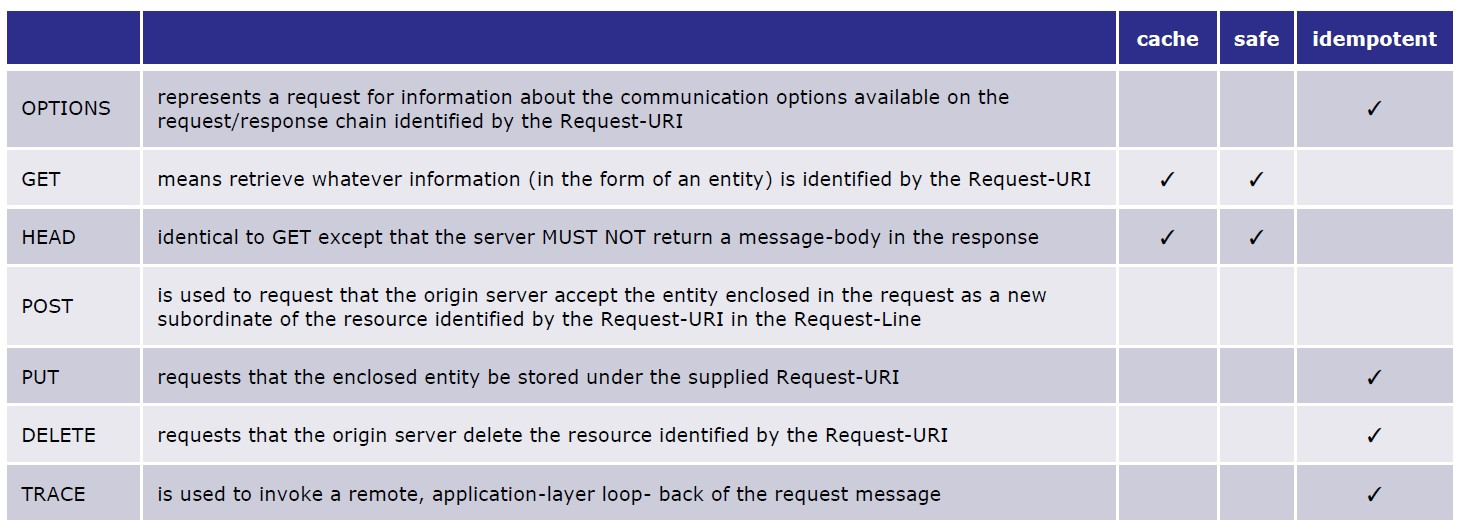
\includegraphics[width=0.675\textwidth]{img/MOC_metodi1.jpg}
\end{center}
\textbf{Safe} = methods SHOULD NOT have the significance of taking an action other than retrieval.
\\\textbf{Idempotent} = the side-effects of N > 0 identical requests is the same as for a single request (aside from error or expiration issues).

\subsection{Formato dei messaggi http}
Messaggio http response
\begin{center}
    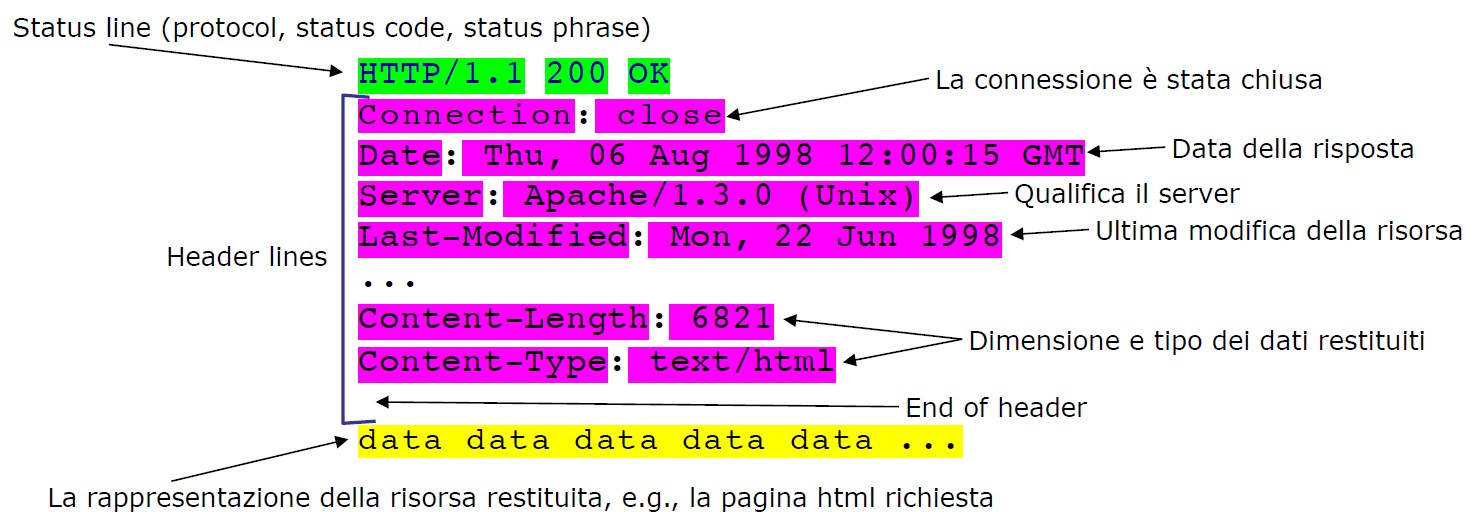
\includegraphics[width=0.675\textwidth]{img/MOC_messaggi3.jpg}
\end{center}
HTTP 1.0: Server chiude connessione al termine della richiesta
\\HTTP 1.1: mantiene aperta la connessione oppure chiude se la richiesta contiene Connection: close
\\
\\Domanda:
\\Perché sono state inserite le informazioni sulla dimensione e il tipo dei dati restituiti?
\begin{verbatim}
    Content-Length: 6812
    Content-Type: text/html
\end{verbatim}








